\newpage

\chapter{Lecture 18/03/2025}




\subsubsection{Polar Coordinates}

Let's consider data disposed as in figure:

\begin{figure}[H]
    \centering
    \includegraphics[width=0.25\textwidth]{assets/polar.png}
    \label{fig:polar}
\end{figure}

We can convert the data from Cartesian to Polar coordinates as follows:

\begin{center}
    \begin{minipage}{0.4\textwidth}
        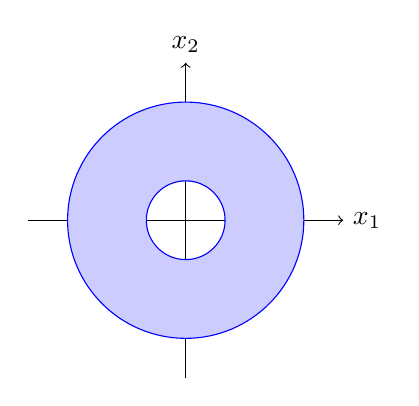
\begin{tikzpicture}[scale=0.5]
            % Draw x and y axes
            \draw[->] (-4,0) -- (4,0) node[right] {$x_1$};
            \draw[->] (0,-4) -- (0,4) node[above] {$x_2$};
            
            % Draw the annulus (circular corona)
            \filldraw[fill=blue!20, draw=blue, even odd rule] 
                (0,0) circle (3cm) (0,0) circle (1cm);
        \end{tikzpicture}
    \end{minipage}
    \begin{minipage}{0.4\textwidth}
        $$
        \begin{cases}
            x_1 \\
            x_2
        \end{cases}
        \quad \rightarrow \quad
        \begin{cases}
            r = \sqrt{x_1^2 + x_2^2} \\
            \theta = arctg \dfrac{x_2}{x_1}
        \end{cases}
        $$
    \end{minipage}
\end{center}

\subsubsection{Other Non-Linearities}

\begin{figure}[H]
    \centering
    \includegraphics[width=0.7\textwidth]{assets/non-lin.png}
\end{figure}


\section{Universal Approximation Theorem}

Let $\sigma$ be any continuous discriminatory function.

$$
\displaystyle
\text{Then finite sums of the form}
\quad
G(x) = \sum_{j=1}^{N} \alpha_j \sigma(y_i^\top x + \theta_j)
\quad
\text{are dense in} C(I_n).
$$ 

In other words, given any $f \in C(I_n)$ and $\varepsilon > 0$, there is a sum, $G(x)$, of the above form, for wich:

$$
|G(x) - f(x)| < \varepsilon \quad \quad \forall x \in I_n
$$

---

Any function $f(x)$ on $\mathbb{R}^d$ with some smoothness conditions can be approximated by a single hidden layer sigmoidal neural network $f_n(x)$ with $n$ hidden units such that:

$$
\int_{B_r} \left(f(x)-f_n(x)\right)^2 \mu(dx) \le \dfrac cn
$$

where $\mu$ is a probability measure on ball $B_r = \{x:|x| < r\}$, $c$ is a constant independent of $n$ and $r$.

\begin{observationblock}[Feature Learning Advantage]

A result of the Universal Approximation Theorem is that no linear combinain of $n$ fixed basis functions yells integrated square error smaller than order:
$$
\left( \dfrac 1n \right) ^ \frac 2d
$$

\end{observationblock}

\section{Number of Linear Regions}

Be $D_i$ the size of the input layer, $D$ the size of the hidden layer, Then, given $D_i \le D$. 

The number of linear regions $N$ is given by:

$$
N \le \sum_{j=0}^{D_i} \binom{D}{j}
$$

\begin{exampleblock}
    Let's consider $D_i = 2$ and $D = 3$. The number of linear regions is given by:

    \begin{minipage}{0.65\textwidth}
        $$
        N \le \binom{3}{0} + \binom{3}{1} + \binom{3}{2} = 1 + 3 + 3 = 7
        $$
    \end{minipage}%
    \begin{minipage}{0.3\textwidth}
        \begin{figure}[H]
            \centering
            \includegraphics[width=0.8\textwidth]{assets/regions.png}
        \end{figure}
    \end{minipage}
\end{exampleblock}

\subsubsection{Fixed Functions}



% \begin{center}
%     \begin{tikzpicture}[x=2cm, y=1.5cm, every node/.style={circle, draw, minimum size=1cm}]
%         % Input layer (2 neurons)
        
%         % Hidden layer (3 neurons)
%         \foreach \j in {1,...,3} {
%             \node[] (H\j) at (1.5,-\j) {$B_{\j}(x)$};
%         }
            
%         \node[] (1) at (0,-1.5) {$\ $};

%         % Connect input layer to hidden layer
%         \foreach \i in {1,2} {
%             \draw[->] (H\i) -- (1);
%         }
%     \end{tikzpicture}
% \end{center}


$$
y = \sum_{w_i} \phi(W_{i_{D_i}} x_{D_i} + b_i) \sim \left\{B_i(x)\right\}
$$

\subsubsection{Polynomial case}

If the dimension is $DIM = 1$ we have something of the form:
$$
y = w_0 + w_1 x + w_2 x^2 + \dots + w_M x^M
$$

If the dimension is $DIM = D$, we have:

$$
y = w_o + \sum_{i = 1}^D w_ix_i + \sum_{i,j = 1}^D w_{ij}x_ix_j + \dots + \sum_{i_1, \dots, i_D = 1}^D w_{i_1, \dots, i_D}x_{i_1} \dots x_{i_D}
$$

The consequence is that the number of parameters grows exponentially with the dimension.

\subsubsection{Curse of dimensionality}

$$
B_i(x) = 
\begin{cases}
    0 & \text{if $x$ does not face in the block $b_i$}\\
    majority & \text{if the class of $x$ in the block $ A$}
\end{cases}
$$
